% !TEX root = ../../../main.tex
% 来源：中学数学实验教材·第二册（几何）
% 章节：直线形 / 三角形
% 原始文件：3.tex，行 646-653
% 类型：tikz
% ---
    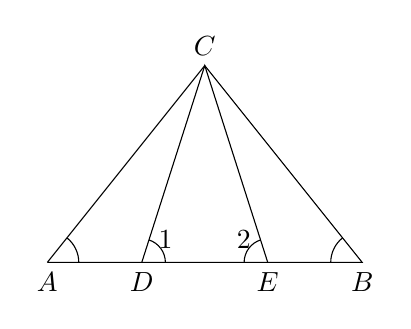
\begin{tikzpicture}[>=latex, scale=1]
\draw(-2,0)node[below]{$A$}--(0,2.5)node[above]{$C$}--(2,0)node[below]{$B$}--(-2,0);
\draw(.8,0)node[below]{$E$}--(0,2.5)--(-.8,0)node[below]{$D$};
\draw (-2+.4,0) arc (0:51.34:.4);
\draw (2-.4,0) arc (180:180-51.34:.4);
\draw (-.8+.3,0) arc (0:72.3:.3)node[right]{1};
\draw (.8-.3,0) arc (180:180-72.3:.3)node[left]{2};
    \end{tikzpicture}
